
\section{Optimization}


\begin{frame}{}
    \tableofcontents[currentsection]
\end{frame}

\subsection{Optimization Problem Formulation}

\begin{frame}{Optimization Problem Formulation}

A multi-objective optimization problem in its more general form can be defined as:
\begin{equation}\label{optiprob}
    \begin{aligned}
        \text{min} \quad & \mathbf{f}(\mathbf{x})=(f_1(x),f_2(x),...,,f_k(x)) \\
        \text{subject to} \quad & \mathbf{H(x)} = 0 \\
        & \mathbf{G(x)} \leq 0
    \end{aligned}
\end{equation}
\begin{itemize}
    \item $\mathbf{x} \in \mathbb{R}^n$: $n$-decision variables.
    \item $\mathbf{f}(\mathbf{x})$: $k$-objective functions.
    \item $\mathbf{H(x)}$: Equality constraints.
    \item $\mathbf{G(x)}$: Inequality constraints.
\end{itemize}


\end{frame}

\begin{frame}{Decision Variables}

We can get the $\mathbf{x}$ variables from the parameters on which the transmission system model ($\mathbf{Y}_{bus}$) depends on:
\begin{equation}\label{vecunk}
    \resizebox{0.9\textwidth}{!}{%
    $\mathbf{x} = 
    \begin{bmatrix}
    vol_{tr}, & n_{cables}, & react_{bi_1}, &, ... &, react_{bi5}&, react_{cont1}&, ... &,react_{cont5}&, react_{bi5}&, S_{trafo}  
    \end{bmatrix}$
    }
\end{equation}

\begin{itemize}
    \item $vol_{tr}$: Transmission voltage level.
    \item $n_{cables}$: Number of transmission cables placed in parallel.
    \item $react_{bi_i}\quad \forall i=1,...,5$: Is a binary variable (i.e. either 0 or 1) that tells if we place or not a reactor at position $i$.
    \item $react_{cont_i} \quad \forall i=1,...,5$: Sizing of reactor at position $i$, therefore its $Y_{sh_{i}}$ in p.u.
    \item $S_{trafo}$: Rated power of the transformer in VA.
\end{itemize}
\vspace{1cm}
\textbf{Mixed-variable:} Continous, binary and integer variables.
\end{frame}



\begin{frame}{Equality Constraints: Power Flow}

The equality constraints $ \mathbf{H(x)} = 0$ in the optimization problem  are the imposed by the power flow equations. In fact, the power mismatch vector takes the desired form:

\begin{equation}
    \mathbf{H(x)} = \begin{bmatrix}
    \mathbf{\Delta P(\mathbf{x})} \\
    \mathbf{\Delta Q(\mathbf{x})}
    \end{bmatrix} = \begin{bmatrix}
    P_1(\mathbf{x}) - P_1 \\
    \vdots \\
    P_{n-1}(\mathbf{x}) - P_{n-1} \\
    Q_1(\mathbf{x}) - Q_1 \\
    \vdots \\
    Q_{n-1}(\mathbf{x}) - Q_{n-1}
    \end{bmatrix} = \mathbf{0}
\end{equation}
    
\end{frame}

\begin{frame}{Inequality Constraints: Technical requirements}

%We want them to take the form of $\mathbf{G(x)} \leq 0$, therefore we can write them as:

\textbf{Bus voltage limits:}
We set the nodal bus-$i$ voltage, $V_i$, limits as:
\begin{equation}
\begin{aligned}
    L_{i}^{Vu} &= V_i - V_{max} \leq 0, \quad i \in N \quad \text{is the upper limit} \\
    L_{i}^{Vl} &= V_{min} - V_i \leq 0, \quad i \in N \quad \text{is the lower limit}   
\end{aligned}    
\end{equation}
We have taken $V_{max}$ and $V_{min}$ to be $\pm 0.1$ p.u. of the nominal voltage respectively.\\

\textbf{Maximum current limits for the lines:}
\begin{equation}
    L_{i}^{I} = I_i - I_{max} \leq 0, \quad i \in N_{lines}
\end{equation}
where $I_{max} = 1.1$ p.u. of $I_{rated}$.

\textbf{Reactive power delivered to the grid:}
\begin{equation}
\begin{aligned}
    L_{6}^{Qu} = Q_6 - Q_{max} \leq 0 \\
    L_{6}^{Ql} = Q_{min} - Q_{6} \leq 0
\end{aligned}
\end{equation}
where we have taken $Q_{max}=Q_{min}=0$, but they can be set by grid code requirements.

\end{frame}

\begin{frame}{Objective Function I}

We want to get insight on the trade-off between conflicting objectives, therefore we will use a multi-objective optimization approach. We will define the objective functions as:

\begin{equation}
    \mathbf{f}(\mathbf{x}) =(f_{invest}(\mathbf{x}),f_{tech}(\mathbf{x}))
\end{equation}
where:
\begin{equation}
\begin{aligned}
    f_{invest}(\mathbf{x}) &= C_{cables}(\mathbf{x}) + C_{tr}(\mathbf{x}) + C_{sh}(\mathbf{x}) + C_{gis-AC}(\mathbf{x}) + C_{ss-AC}(\mathbf{x}) \\
    f_{tech}(\mathbf{x}) &= C_{loss-AC}(\mathbf{x}) + c \cdot \mathbf{p(x)} \\
\end{aligned}
\end{equation}
$c$ is the penalty factor and $\mathbf{p(x)}$ is the penalty function:
\begin{equation}
    \mathbf{p(x)} = \sum_{L_i^X \in G(x)} \max(0, \mathbf{L_i(x)})
\end{equation}

\end{frame}

\begin{frame}{Objective Function II}
With this approach we expect to get a set of Pareto optimal solutions, i.e. a set of solutions where we cannot improve one objective without worsening another:

\begin{figure}
    \centering
    \scalebox{0.65}{
    \includegraphics[width=\textwidth]{imatges/domination.png}
    }
    \caption{Explanation of domination [\textit{check memory for citation}] .}
    \label{fig:domination}
\end{figure}

\end{frame}



\begin{frame}{What we need?}
We need an optimization method that:
\begin{itemize}
    \item Can handle mixed-variable problems.
    \item Can handle multi-objective problems.
    \item Can handle non-linear optimization problems.
    \item Can handle find a set of Pareto optimal solutions, i.e. works with a population of solutions.
\end{itemize}
\vspace{1cm}
PROPOSAL: \textbf{NSGA-II: Non-dominated Sorting Genetic Algorithm II}.
\end{frame}


\subsection{NSGA-II Genetic Algorithm}

\begin{frame}{NSGA-II Genetic Algorithm}
\begin{figure}[H]
    \begin{minipage}{0.45\textwidth}
        \centering
        \scalebox{0.35}{
        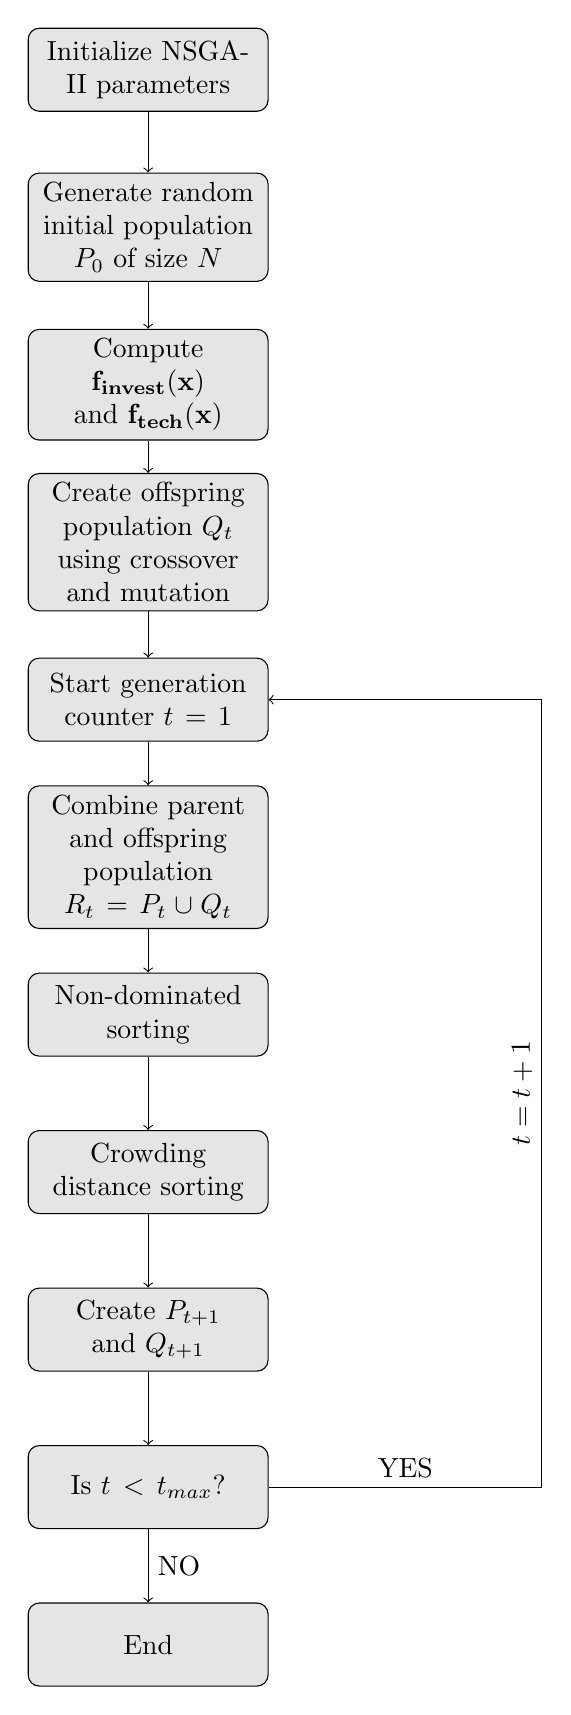
\begin{tikzpicture}[node distance=2cm, auto]
            % Define the style for the boxes
            \tikzstyle{block} = [rectangle, draw, fill=gray!20, 
                                text centered, rounded corners, minimum height=3em, text width= 8em]
        
            \tikzstyle{block3a} = [rectangle, draw, fill=gray!20, 
                                text centered, rounded corners, minimum height=3em, text width=6cm]
        
            % Define the style for the ellipses
            \tikzstyle{block?} = [rectangle, draw, fill=gray!80, 
                                text centered, rounded corners, minimum height=3em, text width=6cm]
        
        
            % Define the nodes
            \node [block] (box1) {Initialize NSGA-II parameters};
            \node [block, below of=box1] (box2) {Generate random initial population $P_0$ of size $N$};
            \node [block, below of=box2] (box3) {Compute $\mathbf{f_{invest}(x)}$ and $\mathbf{f_{tech}(x)}$};
            \node [block, below of=box3] (box4) {Create offspring population $Q_t$ using crossover and mutation};
            \node [block, below of=box4] (box5) {Start generation counter $t=1$};
            \node [block, below of=box5] (box6) {Combine parent and offspring population $R_t = P_t \cup Q_t$};
            \node [block, below of=box6] (box7) {Non-dominated sorting};
            \node [block, below of=box7] (box71) {Crowding distance sorting};
            \node [block, below of=box71] (box72) {Create $P_{t+1}$ and $Q_{t+1}$};
            \node [block, below of=box72] (box8) {Is $t<t_{max}$?};
            \node [block, below of=box8] (box9) {End};
            % Connect the nodes
            \draw [->] (box1) -- (box2);
            \draw [->] (box2) -- (box3);
            \draw [->] (box3) -- (box4);
            \draw [->] (box4) -- (box5);
            \draw [->] (box5) -- (box6);
            \draw [->] (box6) -- (box7);
            \draw [->] (box7) -- (box71);
            \draw [->] (box71) -- (box72);
            \draw [->] (box72) -- (box8);

            \draw [->] (box8) -- node[midway, right] {NO} (box9);
            
            %\draw [->] (box7) to[bend right=80] node[midway,below,sloped] {Optimization method} (box2);
            \draw [->] (box8) -- ++(5,0) node[midway, above] {YES}|-  node[pos=0.25,sloped] {$t=t+1$} (box5);
            
        \end{tikzpicture}
        }
        \caption{NSGA-II algorithm.}
    \end{minipage}
    \begin{minipage}{0.45\textwidth}
        \centering
        \includegraphics[width=\textwidth]{imatges/proces_nsga.png}
        \caption{Sorting and Crowding process [\textit{check memory for citation}].}
        
      \end{minipage}\hfill
    
\end{figure}

\end{frame}

\begin{frame}{Algorithm overview}

    \begin{figure}[h]
        \centering
        \scalebox{0.40}{
        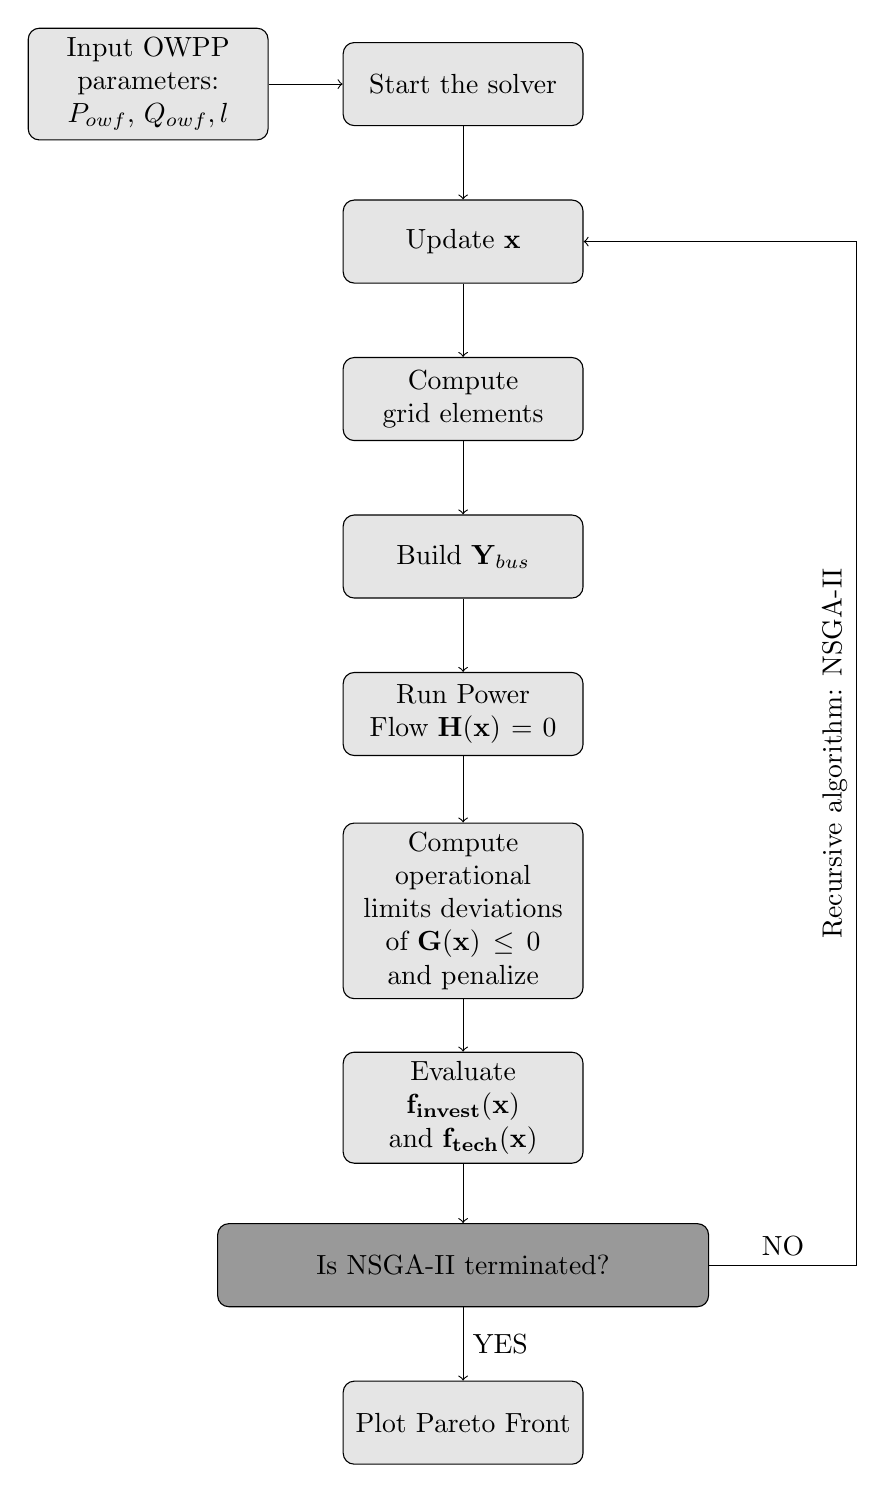
\begin{tikzpicture}[node distance=2cm, auto]
            % Define the style for the boxes
            \tikzstyle{block} = [rectangle, draw, fill=gray!20, 
                                text centered, rounded corners, minimum height=3em, text width= 8em]
        
            \tikzstyle{block3a} = [rectangle, draw, fill=gray!20, 
                                text centered, rounded corners, minimum height=3em, text width=6cm]
        
            % Define the style for the ellipses
            \tikzstyle{block?} = [rectangle, draw, fill=gray!80, 
                                text centered, rounded corners, minimum height=3em, text width=6cm]
        
        
            % Define the nodes
            \node [block] (box1) {Start the solver};
            \node [block, below of=box1] (box2) {Update $\mathbf{x}$};
            \node [block, below of=box2] (box3) {Compute grid elements};
            \node [block, below of=box3] (box4) {Build $\mathbf{Y}_{bus}$};
            \node [block, below of=box4] (box5) {Run Power Flow $\mathbf{H(x)}=0$};
            \node [block, below of=box5, yshift=-0.5cm] (box6) {Compute operational limits deviations of $\mathbf{G(x)} \leq 0$ and penalize};
            \node [block, below of=box6, yshift=-0.5cm] (box7) {Evaluate $\mathbf{f_{invest}(x)}$ and $\mathbf{f_{tech}(x)}$};
            \node [block, left of=box1, xshift=-2cm] (box3a) {Input OWPP parameters: $P_{owf}$, $Q_{owf}, l$};
            \node [block?, below of=box7] (box8) {Is NSGA-II terminated?};
            \node [block, below of=box8] (box9) {Plot Pareto Front};
            % Connect the nodes
            \draw [->] (box1) -- (box2);
            \draw [->] (box2) -- (box3);
            \draw [->] (box3) -- (box4);
            \draw [->] (box4) -- (box5);
            \draw [->] (box5) -- (box6);
            \draw [->] (box6) -- (box7);
            \draw [->] (box3a) -- (box1); % New arrow
            \draw [->] (box7) -- (box8);
            \draw [->] (box8) -- node[midway, right] {YES} (box9);
            
            %\draw [->] (box7) to[bend right=80] node[midway,below,sloped] {Optimization method} (box2);
            \draw [->] (box8) -- ++(5,0) node[midway, above] {NO}|-  node[pos=0.25,sloped] {Recursive algorithm: NSGA-II} (box2);
            
        \end{tikzpicture}
        }
        \caption{Proposed optimization algorithm.}
        \label{fig:block_overview}
        \end{figure}
    
\end{frame}


\subsection{OPF Validation}
\begin{frame}{OPF for reactor sizing validation}

We modify the traditional AC-OPF objective function of minimizing cost of generating active power, $P_G$, for minimizing $C_{sh}$, reactive power compensation cost, while satisfying the constraints:
\begin{equation}\label{eq:Qopf}
    \underset{Q_{sh}}{\text{min}} \quad \mathbf{c_{sh}^T} \mathbf{Q_{sh}} \quad \text{where} \quad \mathbf{c_{sh}} = \begin{bmatrix} K \\ P \\ 0 \end{bmatrix}
    \end{equation}

where $K$ and $P$ come from the cost function of the shunt reactors:
\begin{equation}\label{eq:shuntcost}
    C_{sh}= K \cdot Q_{sh} + P = K \cdot Y_{sh}\cdot U_{AC-N}^2 + P \quad  \text{[M€]} 
\end{equation}

\begin{table}[H]
    \centering
    \begin{tabular}{c|c|c}
    \hline
    \textbf{Location} & \textbf{K} & \textbf{P} \\
    \hline
    Onshore & 0.01049 & 0.8312  \\
    Offshore & 0.01576 & 1.244 \\
    Mid-cable & 0.01576 & 12.44 \\
    \hline
    \end{tabular}
    \caption{K and P for different positions of the shunt reactors [\textit{check memory for citation}].}
    \label{tab:parametersshunt}
    \end{table}
\end{frame}





